\documentclass[11pt,a4paper]{article}

\usepackage[utf8]{inputenc}
\usepackage[T1]{fontenc}
\usepackage[spanish,es-nodecimaldot]{babel}
\usepackage{amsmath}
\usepackage{graphicx}
\usepackage{float}
\usepackage{geometry}
\usepackage{booktabs}
\usepackage{hyperref}

\geometry{margin=2.3cm}
\graphicspath{
  {../outputs/phase1/}
  {../outputs/phase2/}
  {../outputs/phase3/}
  {../outputs/phase4/}
}

\title{Proyecto 2: Clasificaci\'on de Se\~nales Eco-Ac\'usticas}
\author{CS3061 -- Machine Learning}
\date{\today}

\begin{document}

\maketitle

\section{Resumen Ejecutivo e Introducci\'on al Espacio Vectorial}

Se abord\'o el problema de clasificaci\'on automatizada de se\~nales eco-ac\'usticas para apoyar la identificaci\'on de especies faun\'isticas mediante registros preprocesados. Desde una perspectiva ecol\'ogica, una clasificaci\'on confiable permite priorizar revisiones humanas, reducir el costo de monitoreo y acelerar la detecci\'on de presencia biol\'ogica en ambientes con ruido. Matem\'aticamente, cada observaci\'on fue representada como un vector de caracter\'isticas $\mathbf{x}_i \in \mathbb{R}^{64}$, compuesto por los coeficientes \texttt{mel\_0}--\texttt{mel\_63}. La variable objetivo fue \texttt{species\_id}, acotada a las clases $\{10,12,17,18,23\}$.

Se utilizaron estrictamente los archivos \texttt{eco\_acoustic\_train.csv} y \texttt{eco\_acoustic\_test.csv}. El conjunto de entrenamiento contuvo 1906 observaciones y el conjunto de prueba contuvo 477 observaciones. Las variables \texttt{recording\_id}, \texttt{songtype\_id} e \texttt{is\_tp} fueron conservadas como metadatos, pero los modelos fueron ajustados con el espacio MFCC. La arquitectura general del pipeline se resume en la Figura~\ref{fig:arquitectura}.

\begin{figure}[H]
\centering
\fbox{
\begin{minipage}{0.95\textwidth}
\centering
\texttt{eco\_acoustic\_train.csv} / \texttt{eco\_acoustic\_test.csv}\\[0.2cm]
$\downarrow$\\[-0.05cm]
Validaci\'on de columnas \texttt{mel\_0}--\texttt{mel\_63} y etiquetas \texttt{species\_id}\\[0.2cm]
$\downarrow$\\[-0.05cm]
Estandarizaci\'on con media cero y varianza unitaria\\[0.2cm]
$\downarrow$\\[-0.05cm]
Exploraci\'on geom\'etrica: PCA, t-SNE y m\'etricas de preservaci\'on\\[0.2cm]
$\downarrow$\\[-0.05cm]
Miner\'ia no supervisada: GMM y DBSCAN con validaci\'on interna\\[0.2cm]
$\downarrow$\\[-0.05cm]
Clasificaci\'on supervisada: MLP TensorFlow vs. ensamble de \'arboles\\[0.2cm]
$\downarrow$\\[-0.05cm]
Inferencia probabil\'istica y zonas operativas de confianza, incertidumbre y rechazo
\end{minipage}
}
\caption{Arquitectura del pipeline desde la ingesta del CSV hasta la decisi\'on operacional basada en probabilidades.}
\label{fig:arquitectura}
\end{figure}

\section{Exploraci\'on Geom\'etrica y Reducci\'on de Dimensionalidad}

Se estandarizaron las 64 variables continuas antes de aplicar reducci\'on de dimensionalidad, debido a que PCA y t-SNE son sensibles a la escala de entrada. Se ajust\'o PCA completo para estimar la varianza acumulada y se determin\'o que 11 componentes fueron suficientes para alcanzar el 95\% de varianza. Posteriormente, se compar\'o PCA 2D contra t-SNE 2D como aproximaci\'on no lineal de variedades. La comparaci\'on cuantitativa se presenta en la Tabla~\ref{tab:dimensionalidad}.

\begin{table}[H]
\centering
\caption{Comparaci\'on cuantitativa entre PCA y t-SNE.}
\label{tab:dimensionalidad}
\begin{tabular}{lrrrr}
\toprule
M\'etodo & Tiempo (s) & Varianza 2D & Trustworthiness@10 & Corr. distancias \\
\midrule
PCA 2D & 0.003 & 0.671 & 0.867 & 0.947 \\
t-SNE 2D & 20.365 & N/A & 0.987 & 0.590 \\
\bottomrule
\end{tabular}
\end{table}

La proyecci\'on PCA conserv\'o una mayor correlaci\'on global de distancias, mientras que t-SNE preserv\'o mejor la estructura local de vecindarios. Este comportamiento fue consistente con la naturaleza de ambos m\'etodos: PCA optimiza una proyecci\'on lineal asociada a varianza global, mientras que t-SNE prioriza relaciones locales no lineales. La separaci\'on visual por \texttt{species\_id} se muestra en la Figura~\ref{fig:pca-tsne}.

\begin{figure}[H]
\centering
\includegraphics[width=0.95\textwidth]{phase1_embeddings.png}
\caption{Comparaci\'on visual entre PCA 2D y t-SNE 2D para las cinco especies.}
\label{fig:pca-tsne}
\end{figure}

La evoluci\'on de la varianza acumulada de PCA y la diferencia temporal entre m\'etodos se muestran en la Figura~\ref{fig:pca-diagnostico}. Esta evidencia justific\'o el uso de PCA como referencia lineal interpretable y de t-SNE como herramienta exploratoria para estructura local.

\begin{figure}[H]
\centering
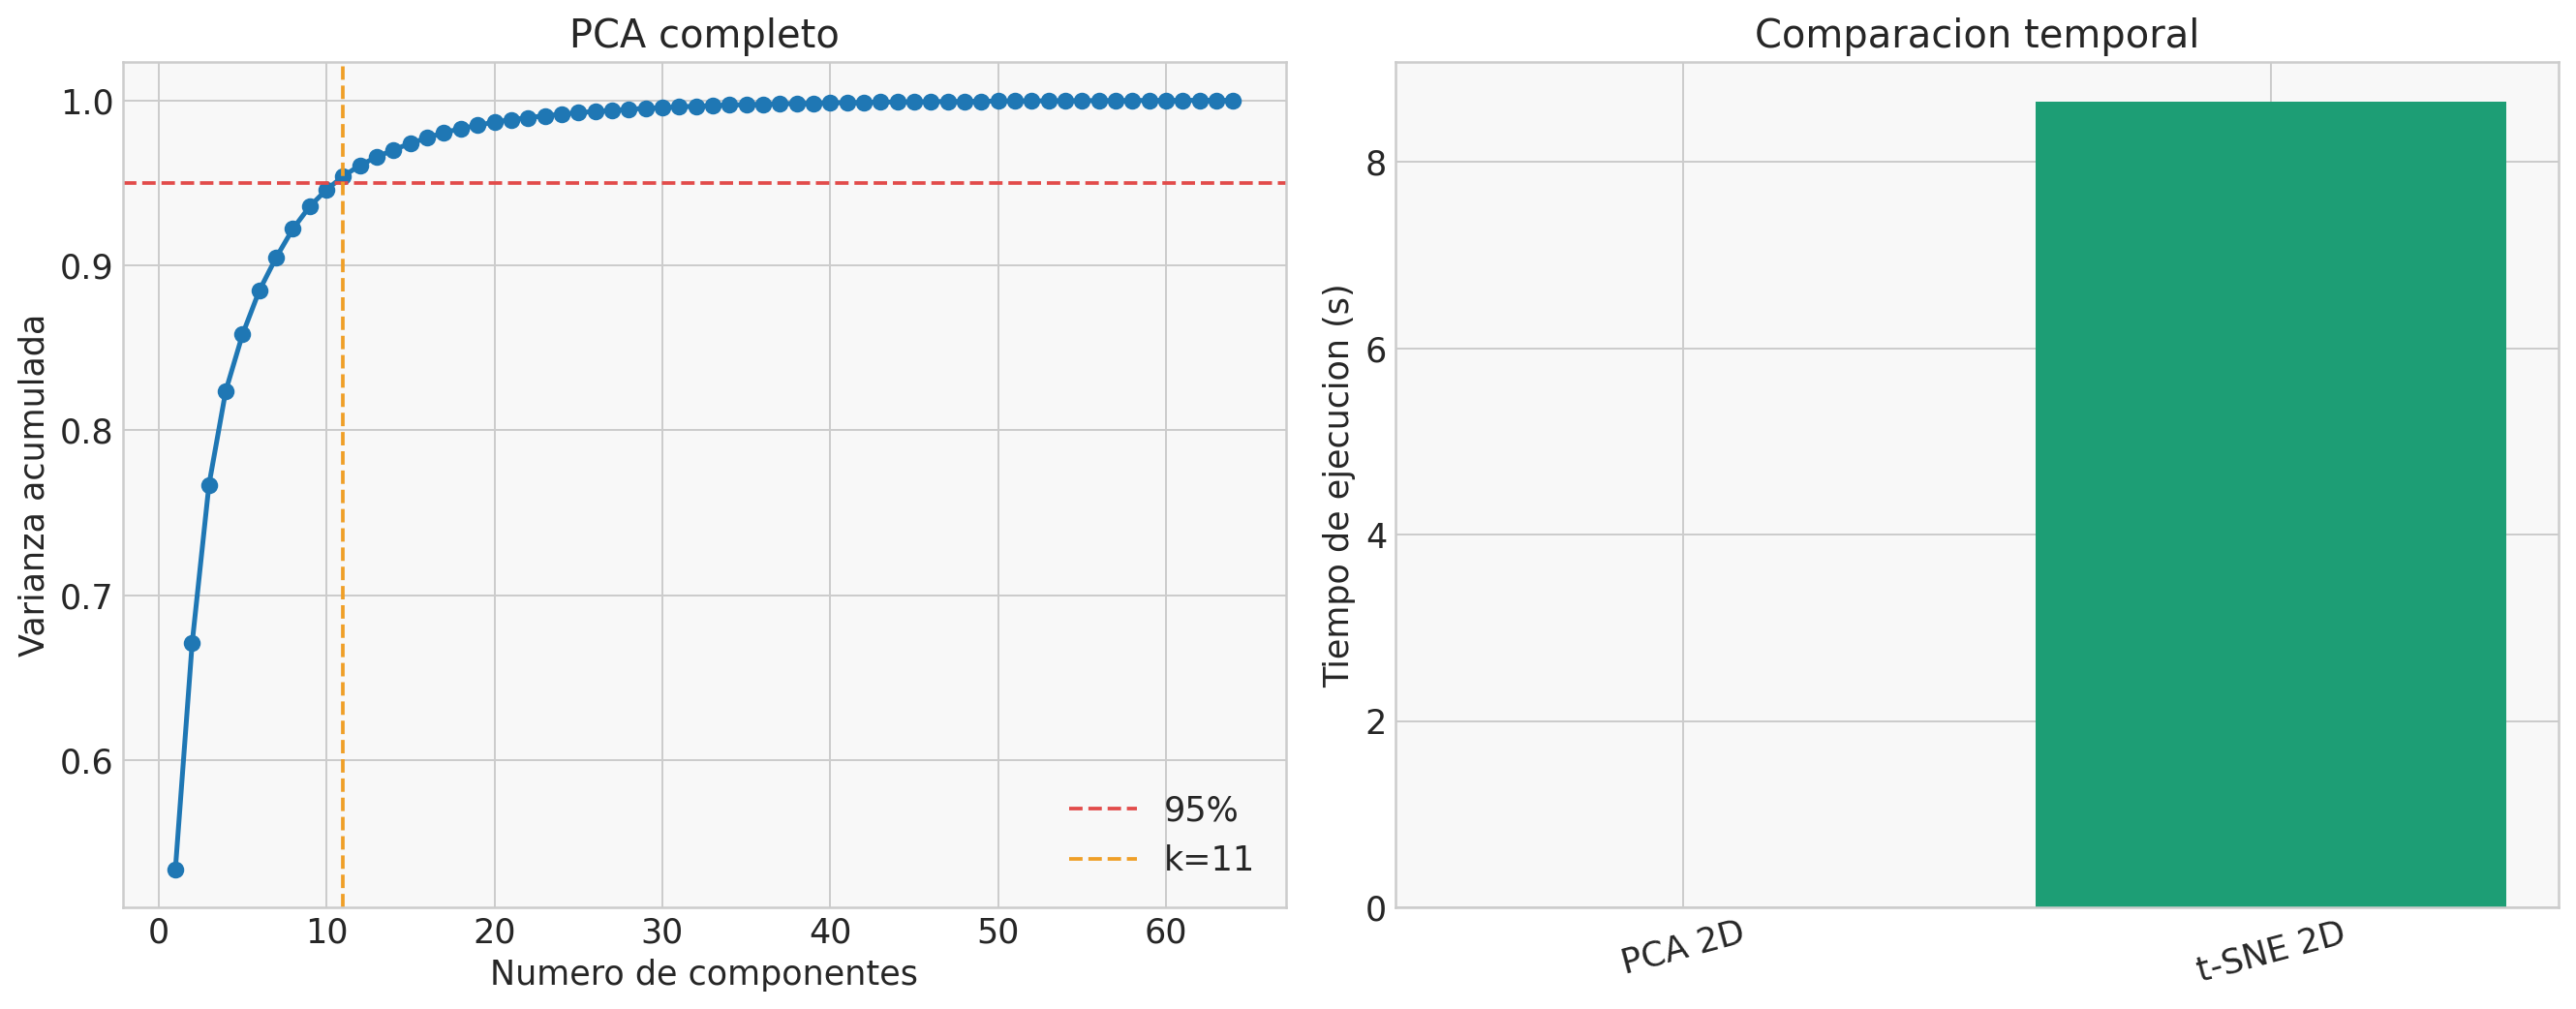
\includegraphics[width=0.90\textwidth]{phase1_diagnostics.png}
\caption{Varianza acumulada de PCA y comparaci\'on temporal entre m\'etodos de reducci\'on.}
\label{fig:pca-diagnostico}
\end{figure}

\section{Miner\'ia de Patrones y Estructuras de Clustering}

Se aplicaron dos paradigmas no supervisados sobre la representaci\'on PCA que retuvo 95\% de varianza: Gaussian Mixture Models (GMM), como modelo probabil\'istico, y DBSCAN, como m\'etodo basado en densidad. Para GMM se evalu\'o una grilla de valores de $k$, mientras que para DBSCAN se exploraron valores de $\varepsilon$ derivados de distancias al vecino m\'as cercano. La Tabla~\ref{tab:clustering} resume los modelos seleccionados.

\begin{table}[H]
\centering
\caption{Selecci\'on de modelos de clustering con m\'etricas internas y diagn\'ostico externo.}
\label{tab:clustering}
\resizebox{\textwidth}{!}{
\begin{tabular}{llrrrrrr}
\toprule
M\'etodo & Par\'ametro & Clusters & Silhouette & DBI & CH & Ruido & ARI \\
\midrule
GMM & $k=2$ & 2 & 0.184 & 1.992 & 382.1 & 0.000 & 0.026 \\
DBSCAN & $\varepsilon=4.488$, \texttt{min\_samples}=10 & 2 & 0.436 & 0.604 & 53.3 & 0.056 & 0.004 \\
\bottomrule
\end{tabular}
}
\end{table}

El coeficiente de Silhouette fue usado como criterio principal, dado que eval\'ua $(b-a)/\max(a,b)$, donde $a$ representa cohesi\'on intra-cluster y $b$ separaci\'on inter-cluster. Como validaci\'on complementaria, se report\'o Davies-Bouldin (DBI), donde valores menores son preferibles, y Calinski-Harabasz (CH), donde valores mayores sugieren mayor separaci\'on relativa. La curva de selecci\'on de hiperpar\'ametros se observa en la Figura~\ref{fig:silhouette}.

\begin{figure}[H]
\centering
\includegraphics[width=0.92\textwidth]{phase2_silhouette_selection.png}
\caption{Selecci\'on de hiperpar\'ametros mediante Silhouette para GMM y DBSCAN.}
\label{fig:silhouette}
\end{figure}

Los agrupamientos no coincidieron de manera fuerte con las clases reales, como se aprecia en la Figura~\ref{fig:clusters}. Por ello, el ARI fue interpretado solamente como diagn\'ostico externo y no como criterio de selecci\'on, ya que las etiquetas \texttt{species\_id} no fueron usadas durante el ajuste no supervisado.

\begin{figure}[H]
\centering
\includegraphics[width=0.92\textwidth]{phase2_clusters_pca2d.png}
\caption{Asignaciones de GMM y DBSCAN visualizadas sobre el plano PCA 2D.}
\label{fig:clusters}
\end{figure}

\section{Arquitectura de Clasificaci\'on: MLP vs. Modelos de ensamble}

Se entren\'o una red neuronal MLP en TensorFlow/Keras y se compar\'o contra un ensamble de \'arboles. La funci\'on de p\'erdida empleada fue la entrop\'ia cruzada categ\'orica dispersa, equivalente a
\[
\mathcal{L} = -\frac{1}{N}\sum_{i=1}^{N}\sum_{c=1}^{5} y_{ic}\log(\hat{p}_{ic}),
\]
donde $y_{ic}$ indica pertenencia a la clase $c$ y $\hat{p}_{ic}$ corresponde a la probabilidad estimada por la capa \textit{softmax}. La topolog\'ia de la red se detalla en la Tabla~\ref{tab:topologia}.

\begin{table}[H]
\centering
\caption{Topolog\'ia del MLP implementado en TensorFlow/Keras.}
\label{tab:topologia}
\begin{tabular}{llr}
\toprule
Bloque & Operaci\'on & Salida \\
\midrule
Entrada & Vector MFCC estandarizado & 64 \\
Oculta 1 & Dense(128) + BatchNorm + ReLU + Dropout(0.30) & 128 \\
Oculta 2 & Dense(64) + BatchNorm + ReLU + Dropout(0.20) & 64 \\
Salida & Dense(5) + Softmax & 5 \\
\bottomrule
\end{tabular}
\end{table}

Para analizar la regularizaci\'on, se compar\'o la configuraci\'on principal con Batch Normalization antes de Dropout contra una variante con Dropout antes de Batch Normalization. Los resultados se reportan en la Tabla~\ref{tab:regularizacion}.

\begin{table}[H]
\centering
\caption{Ablaci\'on del orden relativo entre Batch Normalization y Dropout.}
\label{tab:regularizacion}
\resizebox{\textwidth}{!}{
\begin{tabular}{lrrrr}
\toprule
Variante & \'Epocas & Mejor val-loss & Mejor val-accuracy & Mejor val-F1 ponderado \\
\midrule
BatchNorm $\rightarrow$ ReLU $\rightarrow$ Dropout & 69 & 1.288 & 0.450 & 0.452 \\
Dropout $\rightarrow$ BatchNorm & 41 & 1.254 & 0.463 & 0.436 \\
\bottomrule
\end{tabular}
}
\end{table}

Se observ\'o que la variante con Dropout antes de Batch Normalization redujo la p\'erdida de validaci\'on, pero obtuvo menor F1 ponderado. Por ello, se mantuvo la configuraci\'on principal, ya que la m\'etrica objetivo del problema fue F1-score y no solamente \textit{loss}. Las curvas de aprendizaje del MLP se muestran en la Figura~\ref{fig:curvas}.

\begin{figure}[H]
\centering
\includegraphics[width=0.92\textwidth]{phase3_mlp_learning_curves.png}
\caption{Curvas de p\'erdida, exactitud y F1 ponderado del MLP.}
\label{fig:curvas}
\end{figure}

El modelo de comparaci\'on supervisada fue un ensamble por votaci\'on suave compuesto por Random Forest, Extra Trees e HistGradientBoosting, donde este \'ultimo incorpor\'o \'arboles de decisi\'on por gradiente. La Tabla~\ref{tab:ensamble-val} muestra la validaci\'on de sus componentes.

\begin{table}[H]
\centering
\caption{Desempe\~no de los componentes del ensamble sobre validaci\'on.}
\label{tab:ensamble-val}
\begin{tabular}{lrr}
\toprule
Modelo & F1 ponderado validaci\'on & Tiempo (s) \\
\midrule
Random Forest & 0.443 & 2.230 \\
Extra Trees & 0.422 & 1.346 \\
HistGradientBoosting & 0.422 & 17.665 \\
Soft Voting Ensemble & 0.437 & 20.071 \\
\bottomrule
\end{tabular}
\end{table}

La comparaci\'on final sobre el conjunto de prueba se reporta en la Tabla~\ref{tab:clasificacion}. El ensamble obtuvo mayor exactitud y F1 ponderado, mientras que el MLP obtuvo un F1 macro ligeramente superior, lo cual sugiere una distribuci\'on distinta de errores por clase.

\begin{table}[H]
\centering
\caption{Comparaci\'on de clasificadores sobre el conjunto de prueba.}
\label{tab:clasificacion}
\begin{tabular}{lrrr}
\toprule
Modelo & Accuracy & F1 macro & F1 ponderado \\
\midrule
MLP TensorFlow & 0.451 & 0.451 & 0.450 \\
Soft Voting Ensemble & 0.491 & 0.428 & 0.469 \\
\bottomrule
\end{tabular}
\end{table}

Las matrices de confusi\'on de la Figura~\ref{fig:confusion} evidencian errores de asignaci\'on entre especies ac\'usticamente solapadas. Este resultado justific\'o el uso de F1-score como m\'etrica principal, en lugar de depender exclusivamente de accuracy.

\begin{figure}[H]
\centering
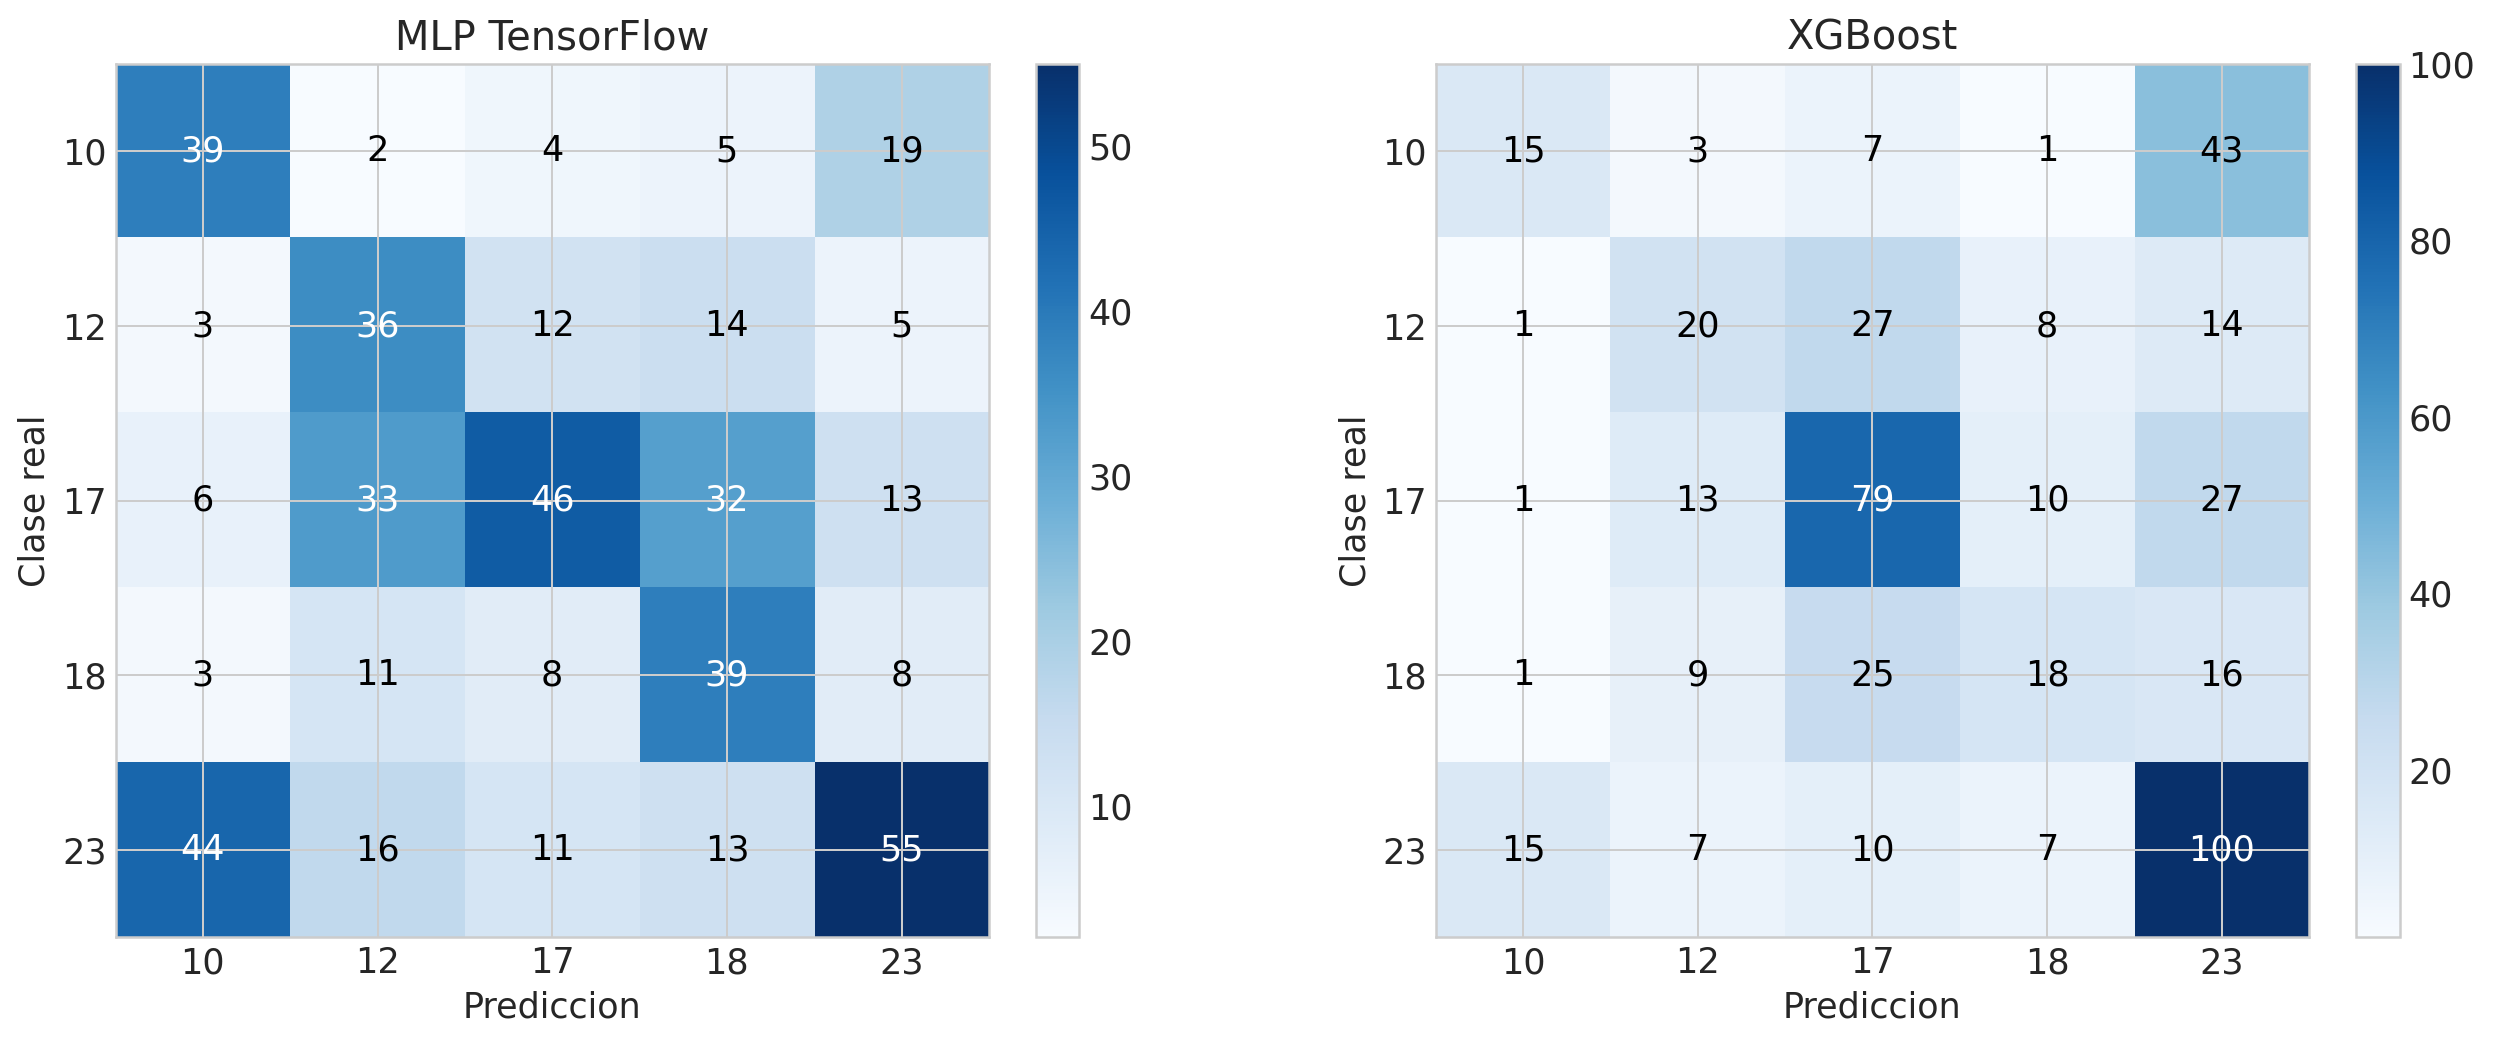
\includegraphics[width=0.92\textwidth]{phase3_confusion_matrices.png}
\caption{Matrices de confusi\'on del MLP y del ensamble sobre el conjunto de prueba.}
\label{fig:confusion}
\end{figure}

\section{Decisiones de Ingenier\'ia y Mitigaci\'on de Riesgos (MLOps \& Negocio)}

Se analiz\'o el compromiso entre costo computacional y rendimiento anal\'itico usando los tiempos medidos en inferencia experimental. El MLP requiri\'o 31.055 s durante entrenamiento y evaluaci\'on, con F1 ponderado de 0.450, mientras que el ensamble requiri\'o 41.312 s y alcanz\'o F1 ponderado de 0.469. Por tanto, el ensamble fue m\'as costoso, pero entreg\'o una mejora absoluta aproximada de 0.018 en F1 ponderado. Dado que la inferencia eco-ac\'ustica puede operar de forma diferida o por lotes, se consider\'o aceptable priorizar el desempe\~no anal\'itico del ensamble.

Sobre la salida probabil\'istica del ensamble se propuso una pol\'itica de tres zonas: confianza, incertidumbre y rechazo. La Tabla~\ref{tab:umbrales} resume la cobertura y desempe\~no de cada zona.

\begin{table}[H]
\centering
\caption{Resumen operativo de zonas de decisi\'on.}
\label{tab:umbrales}
\begin{tabular}{lrrrr}
\toprule
Zona & Observaciones & Cobertura & Accuracy & Prob. media \\
\midrule
Zona de Confianza & 9 & 0.019 & 0.667 & 0.883 \\
Zona de Incertidumbre & 417 & 0.874 & 0.492 & 0.588 \\
Zona de Rechazo & 51 & 0.107 & 0.451 & 0.353 \\
\bottomrule
\end{tabular}
\end{table}

La zona de confianza fue definida para predicciones con $P \geq 0.85$, la zona de incertidumbre para $0.40 \leq P < 0.85$ y la zona de rechazo para $P < 0.40$. La distribuci\'on emp\'irica de probabilidades se presenta en la Figura~\ref{fig:umbrales}. La baja cobertura de la zona de confianza indic\'o que el sistema debe operar con revisi\'on humana frecuente, especialmente cuando se busque mitigar falsos positivos en monitoreo ecol\'ogico.

\begin{figure}[H]
\centering
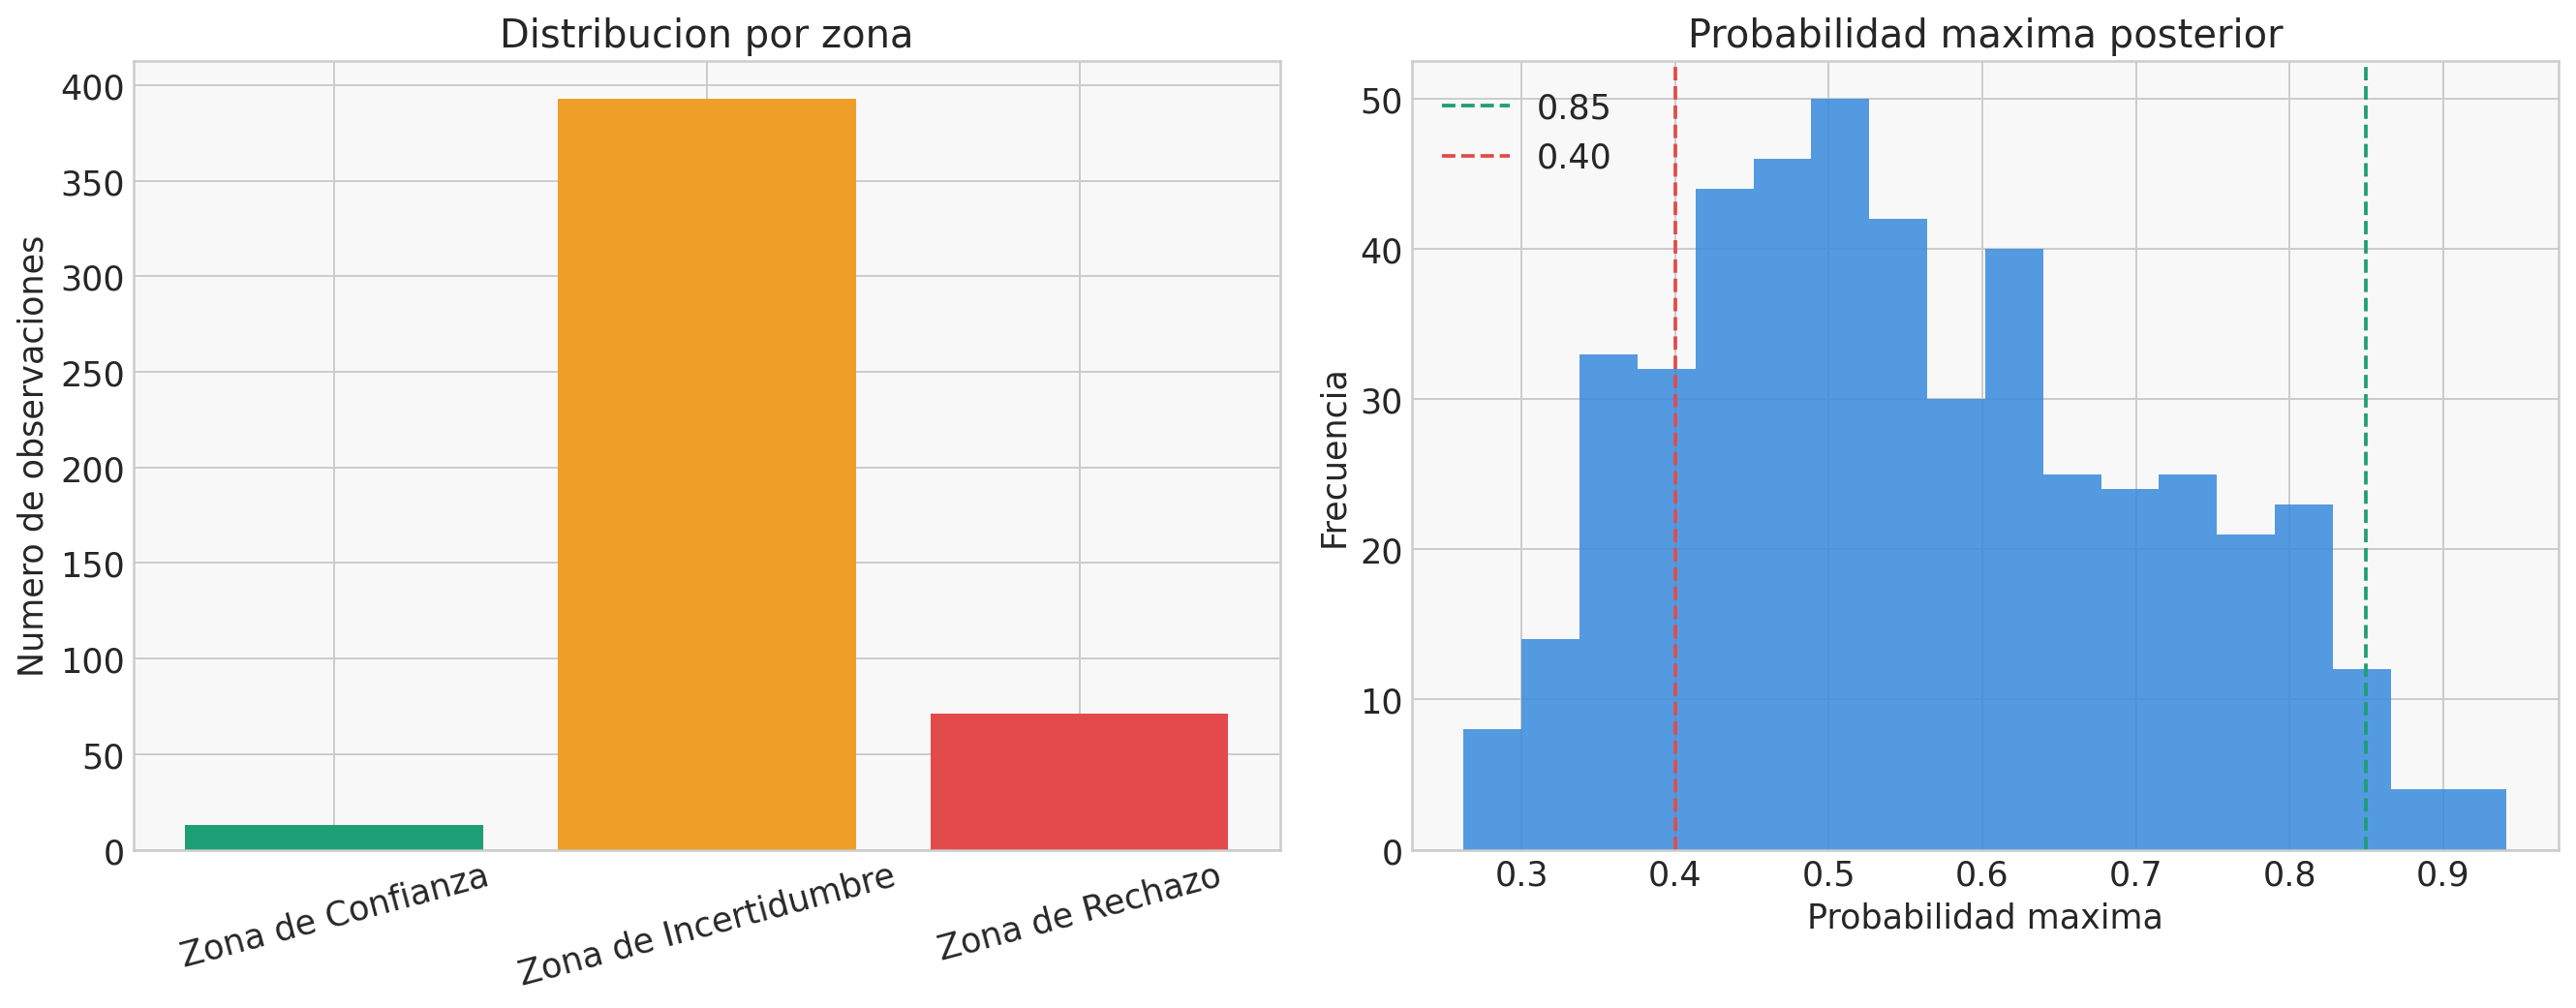
\includegraphics[width=0.90\textwidth]{phase4_threshold_diagnostics.png}
\caption{Distribuci\'on de zonas operativas y probabilidades posteriores m\'aximas.}
\label{fig:umbrales}
\end{figure}

\section{Contribution statement}

La asignaci\'on de responsabilidades del equipo se presenta en la Tabla~\ref{tab:contribucion}. Esta tabla debe actualizarse con los nombres oficiales antes de la entrega si el trabajo fue realizado por m\'as de un integrante.

\begin{table}[H]
\centering
\caption{Matriz de coevaluaci\'on del equipo de desarrollo.}
\label{tab:contribucion}
\begin{tabular}{lrl}
\toprule
Nombre del Integrante & \% Contribuci\'on & Tareas encargadas \\
\midrule
Integrante 1 & 100\% & Pipeline, experimentaci\'on, informe y validaci\'on de resultados \\
Integrante 2 & 0\% & No aplica \\
Integrante 3 & 0\% & No aplica \\
Integrante 4 & 0\% & No aplica \\
\bottomrule
\end{tabular}
\end{table}

\end{document}
